\section{Problem}
A great quantity of information about artists and music exist on the internet, however, depending on the platform visited or the search provider used the data could vary, making the information inconsistent and incorrect.

In general, most of this information comes from private companies that are dedicated to the music business, like Spotify \citep{spotify} or Last.fm \citep{lastfm}, that provide more accurate and correct data but that is not always the case. Moreover, the data is not freely available and is usually being subjected to some conditions, so the correction of it is not an easy or possible task.  

On the contrary, search engines and music platforms also work with the information contained in open data portals, like Wikipedia or MusicBrainz, where a great quantity of the information is crowdsourced and, in the case of music, generated by fans.  

Even though these pages have control mechanisms to verify the data uploaded, is easy to find the problems described previously. For example, there are situations where the genres of a band differ between sites or where some information is missing in some but not others at it can be appreciated in the figure \ref{fig:data-comp}.

\begin{figure}[t!]
	\centering
	\begin{subfigure}{0.46\columnwidth}
		\centering
		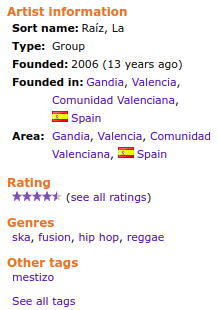
\includegraphics[width=0.7\linewidth]{images/mb-laraiz.png}
		\caption{La Raiz information in MusicBrainz.}
		\label{subfig:raiz_mb}
	\end{subfigure}
	\begin{subfigure}{0.46\columnwidth}
		\centering
		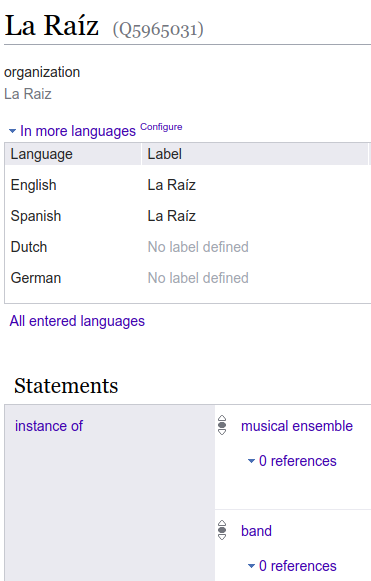
\includegraphics[width=0.63\linewidth]{images/wd-laraiz.png}
		\caption{La Raiz information in MusicBrainz.}
		\label{subfig:raiz_wd}
	\end{subfigure}

	\caption{Comparison between the data of \textbf{a.}MusicBrainz and \textbf{b.}Wikidata.}
	\label{fig:data-comp}
\end{figure}